\begin{figure}[h!]
    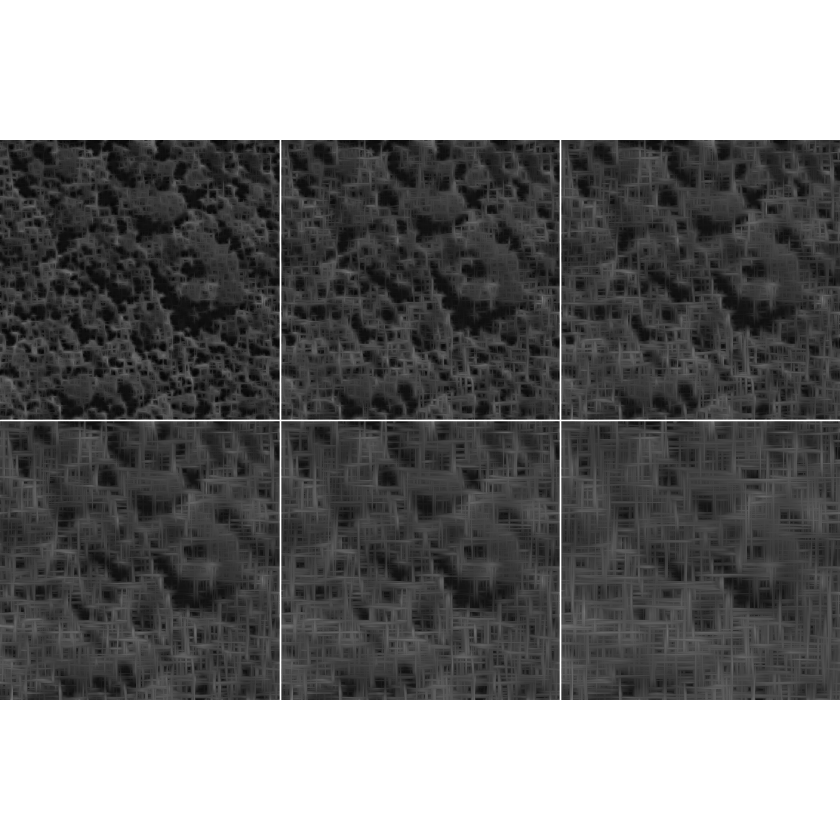
\includegraphics[width=\textwidth]{Imagenes/Resultados script morfologico/GS04.png}
     \hfill
     \caption{Resultado de Rollingball para tamaños de ventana de 6,9,12,15,18 y 24 píxeles}
    \label{Rollingball}
\end{figure}

\begin{figure}[h!]
    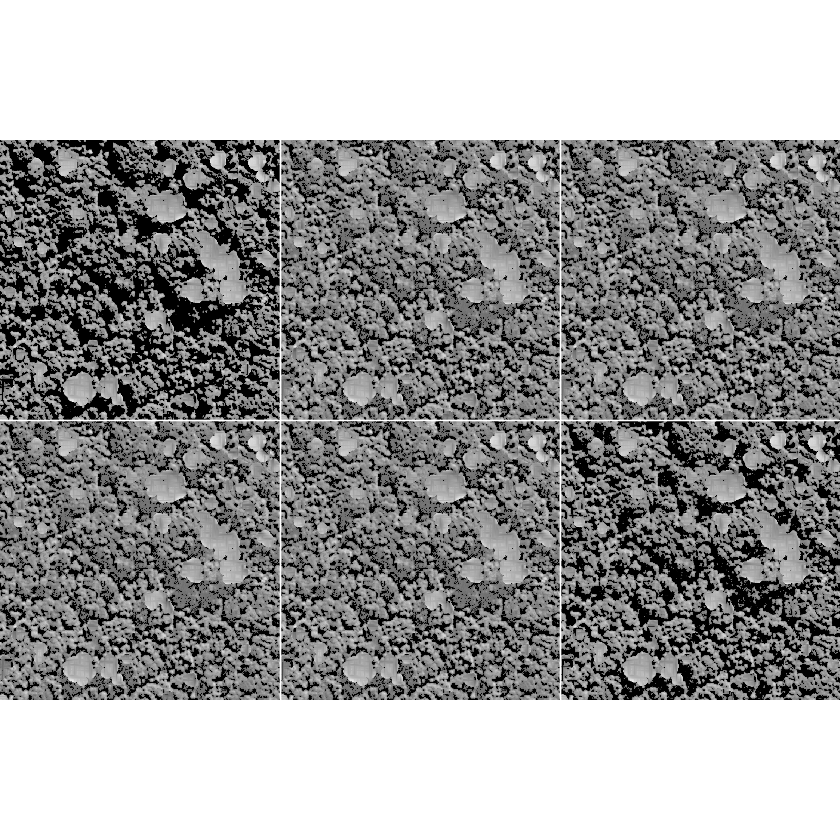
\includegraphics[width=\textwidth]{Imagenes/Resultados script morfologico/GS06.png}
     \hfill
     \caption{Resultado de la segunda selección de objetos oscuros con distintos valores de percentil, 99, 0,1, 1, 10, 50 y 90 }
    \label{segundaoscuros}
\end{figure}

\begin{figure}[h!]
    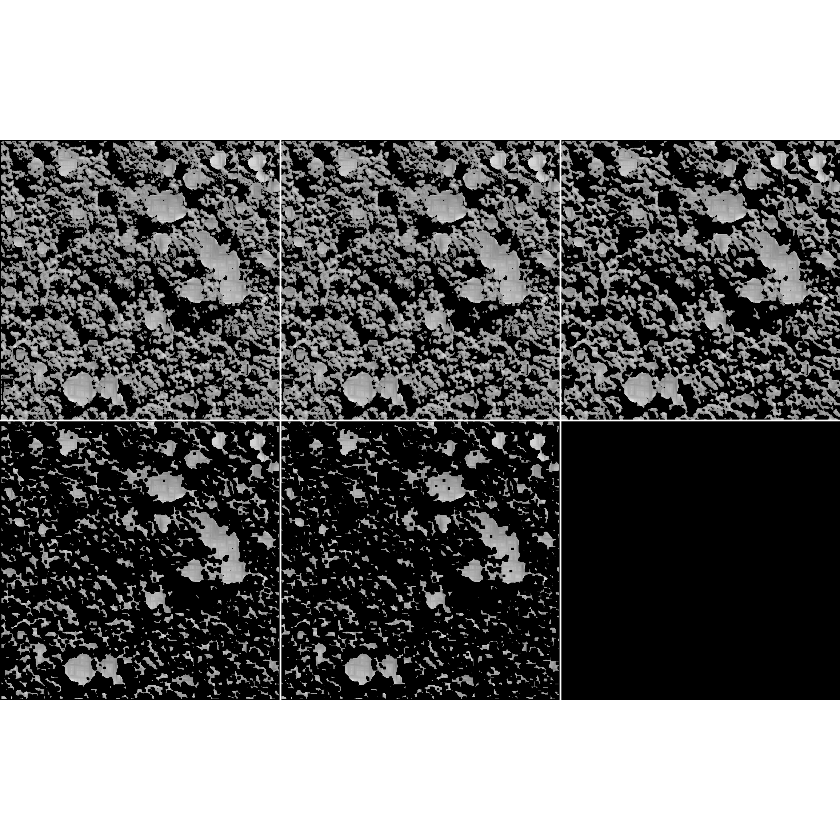
\includegraphics[width=\textwidth]{Imagenes/Resultados script morfologico/GS07.png}
     \hfill
     \caption{Resultado de la búsqueda de pequeños huecos con distintos valores de percentil, 10, 30, 50, 75, 80 y 90 }
    \label{pequenoshuecos}
\end{figure}

\begin{figure}[h!]
    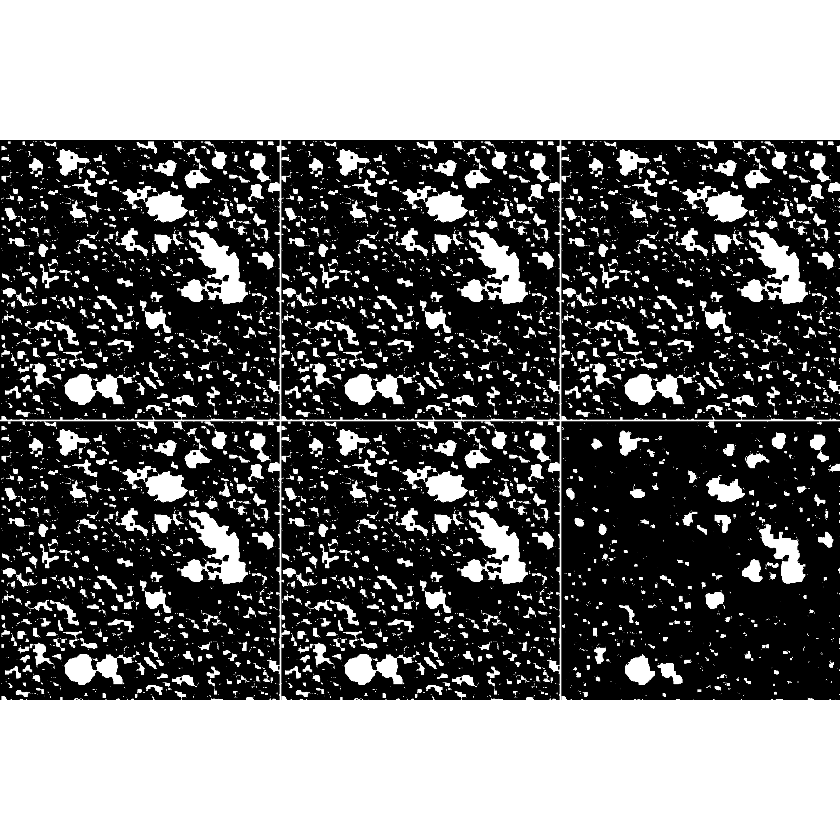
\includegraphics[width=\textwidth]{Imagenes/Resultados script morfologico/GS09.png}
     \hfill
     \caption{Resultado del filtrado con topbottom y binarizado con distintos valores de percentil, 0,1, 1, 10, 20, 50 y 90 }
    \label{topbottom}
\end{figure}